\chapter{Instruction Encoding, Fixups, and Relocatable Objects}
\label{ch:assembly-encoding}

The text \code{call answer} hides two independent decisions.
The assembler must select the x86-64 call encoding and reserve the displacement field.
The linker must later compute the displacement from the final locations of the call and its target.
Correctly choosing opcode \code{E8} does not make an incorrect displacement harmless, and correct address arithmetic does not rescue a wrongly located field.
This chapter joins the two contracts without collapsing them into one undocumented patch operation.

We use little-endian ELF64 objects, explicit-addend relocations, and the instruction subset implemented in \path{example-code/lua-toolchain/luaas.c}.
The generic ELF definitions and the AMD64 relocation definitions are separate specifications~\cite{xinuos-2026-elf,matz-2012-amd64}.
The worked encodings are checked against GNU assembler output; the case study also tests its objects with an independent production linker.

\section{Instruction selection continues inside the assembler}
\label{sec:ch54-forms}

A mnemonic can denote a family of encodings with different operand widths, immediate widths, and addressing modes.
The assembler selects one form after checking operand classes.
For example, moving an immediate into a 64-bit register can use a full 64-bit immediate form, or in suitable cases a shorter sign-extending form.
The case study always uses the full-width form for a 64-bit destination.
This loses some compactness but makes instruction length independent of the eventual value of a symbol.

Writing a 32-bit general-purpose register in 64-bit mode zeroes the upper half of the corresponding 64-bit register.
Consequently, \code{mov eax, 42} is a five-byte way to establish the 64-bit value $42$ in \code{rax}.
It is not interchangeable with every move to \code{rax}: a negative 32-bit bit pattern zero-extends rather than becoming the corresponding negative 64-bit value.
Width is semantics, not merely formatting.

Table~\ref{tab:ch54-bytes} gives exact encodings from the implemented subset.
The hexadecimal byte order is file order, from low to high address.
An immediate such as \code{0x12345678} is serialized least-significant byte first, regardless of the byte order of the host compiling the assembler.

\begin{table}[htbp]
\caption{Concrete instruction forms determine both instruction length and operand semantics.}
\label{tab:ch54-bytes}
\centering
\begin{tabular}{lll}
\toprule
Source operation & Bytes in order & Length \\
\midrule
\code{mov eax, 42} & \code{B8 2A 00 00 00} & $5$ \\
\code{mov edi, eax} & \code{89 C7} & $2$ \\
\code{xor edi, edi} & \code{31 FF} & $2$ \\
\code{syscall} & \code{0F 05} & $2$ \\
\code{ret} & \code{C3} & $1$ \\
\bottomrule
\end{tabular}
\end{table}

\section{Separate opcode bits from operand bits}
\label{sec:ch54-modrm}

For register-to-register \code{mov} in the selected form, opcode \code{89} moves the register encoded in the ModR/M reg field into the operand encoded by r/m.
With both operands registers, the ModR/M mode bits are binary $11$.
For \code{mov edi, eax}, the source register number is zero and destination number is seven, giving
\[
 (3\ll6)\mathbin{\vert}(0\ll3)\mathbin{\vert}7=\texttt{0xC7}.
\]
The assembler's source grammar is destination first, while this particular opcode assigns the source to the reg field.
Blindly mapping the first textual operand into the reg bits reverses the operation.

Figure~\ref{fig:ch54-modrm} illustrates this field assignment.
Other instructions assign different meanings to the same physical fields.
For an immediate arithmetic instruction, the reg field can be an opcode extension rather than a register operand.
The case-study \code{add}, \code{sub}, and \code{cmp} immediate forms use extension values zero, five, and seven respectively.
An encoding table must record operand roles as well as bit positions.

\begin{figure}[htbp]
\centering
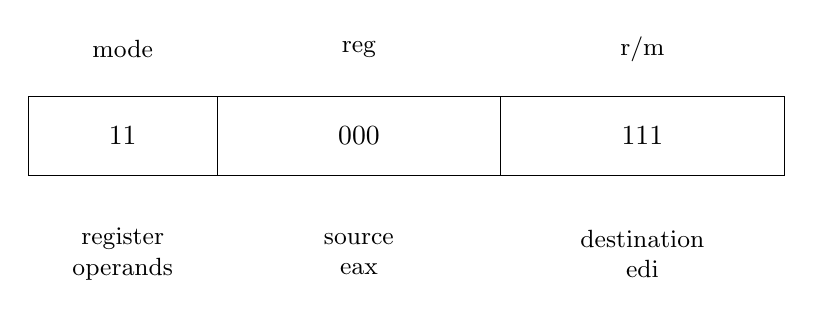
\begin{tikzpicture}[x=12mm,y=10mm]
\draw (0,0) rectangle (2,1); \draw (2,0) rectangle (5,1); \draw (5,0) rectangle (8,1);
\node at (1,0.5) {11}; \node at (3.5,0.5) {000}; \node at (6.5,0.5) {111};
\node[font=\small] at (1,1.6) {mode}; \node[font=\small] at (3.5,1.6) {reg}; \node[font=\small] at (6.5,1.6) {r/m};
\node[font=\small,align=center] at (1,-1) {register\\operands};
\node[font=\small,align=center] at (3.5,-1) {source\\eax};
\node[font=\small,align=center] at (6.5,-1) {destination\\edi};
\end{tikzpicture}
\caption{ModR/M fields describe the chosen opcode form, not a universal ordering of textual operands.}
\label{fig:ch54-modrm}
\end{figure}

For 64-bit operations in this subset, byte \code{48} supplies REX.W.
The first eight registers fit in the existing three-bit fields; extended registers would require REX.R or REX.B according to the operand position.
Memory addressing would add further mode, displacement, and sometimes SIB decisions.
The teaching assembler implements one RIP-relative address-forming operation rather than claiming general ModR/M memory support.
Its rejection of unsupported forms is part of correctness.

\begin{algorithm}[htbp]
\caption{Encode a checked register-to-register instruction form.}
\label{alg:ch54-reg-encode}
\begin{pseudocode}
\Require selected opcode form, destination $d$, source $s$, equal widths
\Ensure bytes implement the form with both operands in the supported register bank
\State require $0\le d<8$ and $0\le s<8$
\If{operand width is 64 bits}
  \State emit REX.W prefix
\EndIf
\State emit the selected opcode byte
\State $m\gets 192+8s+d$
\State emit $m$ as the ModR/M byte
\end{pseudocode}
\end{algorithm}

Algorithm~\ref{alg:ch54-reg-encode} takes constant time for a checked form.
The interesting engineering cost is selecting and validating that form from syntax.
Production assemblers commonly use generated tables to cover instruction families, feature predicates, and diagnostic alternatives.
The case study uses explicit C branches because its supported family is small enough to inspect completely.

\section{A fixup is a deferred field computation}
\label{sec:ch54-fixup-record}

A \term{fixup} records a field whose contents cannot yet be committed.
Its record needs the containing section, byte offset, width or relocation kind, target symbol identity, and addend.
It also needs enough diagnostic context to explain a later failure.
A fixup is not necessarily an object relocation: an assembler can resolve a local fixup after layout, while preserving another as a relocation for the linker.
The case study preserves all supported symbolic fields as ELF RELA entries, including same-section branches.

Consider a call beginning at section offset $17$.
Its opcode occupies offset $17$ and its four-byte displacement occupies offsets $18$ through $21$.
The processor adds the displacement to the address after the instruction, at offset $22$.
ELF's PC-relative relocation convention uses $P$, the address of the relocation field, rather than the address after the instruction.
Therefore the addend includes $-4$:
\[
 D=S+A-P,\qquad A=-4,\qquad P=B_{text}+18.
\]
If the target lands at $B_{text}+32$, then $D=32-4-18=10$.
The processor reconstructs $B_{text}+22+10=B_{text}+32$.
The addend is not the negative length of the entire five-byte call.

\begin{figure}[htbp]
\centering
\begin{tikzpicture}[x=13mm,y=10mm]
\draw (0,0) rectangle (1,1); \node at (0.5,0.5) {E8};
\draw (1,0) rectangle (5,1); \node at (3,0.5) {displacement: 10};
\node[font=\small] at (0,1.5) {17}; \node[font=\small] at (1,1.5) {18: P}; \node[font=\small] at (5,1.5) {22: next RIP};
\draw[cfg edge] (5,-0.5)--node[below,font=\small] {add 10}(8,-0.5);
\node[font=\small] at (8,0.5) {32: target};
\end{tikzpicture}
\caption{The relocation place is the displacement field; the processor's branch base is four bytes later.}
\label{fig:ch54-pcrel}
\end{figure}

The same distinction applies to RIP-relative \code{lea} in the selected form: its displacement ends at the instruction boundary, so its field also receives a $-4$ addend.
An instruction with further bytes after the relocated field can need a different adjustment.
Derive the addend from the actual instruction form rather than copying a constant associated with the mnemonic.

\section{Width checks depend on extension semantics}
\label{sec:ch54-widths}

Truncating an integer to a field width is easy; proving that the truncation preserves the intended value is the actual task.
For an unsigned 32-bit address field, require $0\le V\le2^{32}-1$.
For a sign-extended 32-bit field, require $-2^{31}\le V\le2^{31}-1$.
The same low four bytes can represent different intended values under these contracts.
Table~\ref{tab:ch54-relocations} gives the subset used by the toolchain.

\begin{table}[htbp]
\caption{Relocation formulas and range rules are target-specific contracts, not generic truncation requests.}
\label{tab:ch54-relocations}
\centering
\begin{tabular}{lll}
\toprule
AMD64 relocation & Computation & Field interpretation \\
\midrule
\code{R\_X86\_64\_64} & $S+A$ & full 64-bit result \\
\code{R\_X86\_64\_PC32} & $S+A-P$ & signed 32-bit displacement \\
\code{R\_X86\_64\_32} & $S+A$ & zero-extended 32-bit value \\
\code{R\_X86\_64\_32S} & $S+A$ & sign-extended 32-bit value \\
\code{R\_X86\_64\_PLT32} & $L+A-P$ & displacement to PLT entry \\
\bottomrule
\end{tabular}
\end{table}

Here $L$ denotes a PLT-entry address, not automatically the symbol's address.
Our static linker has no preemptable dynamic definitions and resolves supported PLT32 calls directly to the chosen definition, effectively substituting $S$ for $L$.
That substitution is justified by this link mode; it is not the general PLT32 formula~\cite{matz-2012-amd64}.

Host arithmetic must also be defined.
Computing an overflowing signed sum in C and checking its value afterward is too late.
The implementation checks signed-addition bounds before evaluating the sum for narrow relocations.
Its full-width 64-bit relocation uses unsigned arithmetic modulo $2^{64}$.
Input virtual addresses are restricted to the documented low half of the address space, which makes the intermediate address difference representable in signed 64 bits.

\section{Write ELF records explicitly}
\label{sec:ch54-elf}

An ELF64 relocatable object contains an ELF header, section payloads, string tables, symbol entries, relocation entries, and a section-header table.
The section-header table gives the type, size, offset, alignment, and cross-table links needed to interpret each payload.
The file need not place the table before the data it describes.
Writing it last is convenient because payload offsets are then known.

Do not serialize an in-memory C structure with \code{fwrite} and assume it is a valid disk structure.
Host padding, byte order, alignment, and field widths belong to the host ABI.
The implementation writes each ELF field with an explicit byte width and little-endian order.
Its object reader similarly reads bytes through checked accessors rather than casting an unaligned file pointer to \code{Elf64\_Sym *}.
This makes the on-disk contract inspectable and avoids unaligned-access undefined behavior.

Table~\ref{tab:ch54-records} lists the fixed record sizes relevant here.
These sizes are format facts, not consequences of the compiler's \code{sizeof} for locally declared structures.
Every offset/count pair must be checked against the actual file size before dereferencing the corresponding range.

\begin{table}[htbp]
\caption{ELF64 record widths are serialized independently of host structure layout.}
\label{tab:ch54-records}
\centering
\begin{tabular}{lll}
\toprule
Record & Bytes & Relevant relationship \\
\midrule
ELF header & $64$ & points to section/program tables \\
Section header & $64$ & describes one section \\
Symbol entry & $24$ & names string and defining section \\
RELA entry & $24$ & offset, symbol/type, signed addend \\
Program header & $56$ & describes a runtime segment \\
\bottomrule
\end{tabular}
\end{table}

\section{Cross-table indices are part of correctness}
\label{sec:ch54-indices}

An ELF RELA section's \code{sh\_link} identifies its symbol table and \code{sh\_info} identifies the section to patch.
Each relocation then combines a symbol-table index and a target-specific relocation number in \code{r\_info}.
The symbol table's own \code{sh\_link} identifies its string table.
These are distinct namespaces; a section number is not a symbol number merely because both fit in an integer.
Figure~\ref{fig:ch54-indices} follows one call relocation through those dependencies.

\begin{figure}[htbp]
\centering
\begin{tikzpicture}[node distance=16mm and 24mm]
\node[basic block] (r) {.rela.text};
\node[basic block,right=of r] (s) {.symtab};
\node[basic block,below=of r] (t) {.text: patch field};
\node[basic block,below=of s] (str) {.strtab: answer};
\draw[cfg edge] (r)--node[above=3mm,font=\small] {link + symbol index}(s);
\draw[cfg edge] (r)--node[left,font=\small] {info + offset}(t);
\draw[cfg edge] (s)--node[right,font=\small] {link + name offset}(str);
\end{tikzpicture}
\caption{A relocation reaches its patch location and symbol spelling through different validated index chains.}
\label{fig:ch54-indices}
\end{figure}

\begin{algorithm}[htbp]
\caption{Serialize symbols without invalidating relocation identities.}
\label{alg:ch54-symbol-order}
\begin{pseudocode}
\Require internal symbols with stable identifiers, fixups referencing those identifiers
\Ensure ELF local-first ordering and correct relocation symbol indices
\State emit the all-zero symbol entry at index zero
\ForAll{local symbols, then nonlocal symbols, retaining order within each group}
  \State assign the next ELF index and record $map[internal]\gets index$
  \State emit the symbol name offset, binding, section index, and value
\EndFor
\State record the first nonlocal index in the symbol-table section header
\ForAll{fixups}
  \State translate the internal target through $map$
  \State emit relocation offset, translated symbol/type pair, and addend
\EndFor
\end{pseudocode}
\end{algorithm}

Algorithm~\ref{alg:ch54-symbol-order} is linear in the symbol and relocation counts after names have been interned.
The serializer must additionally account for output bytes and string-table construction.
An empty symbol table still has its null entry; an empty relocation section can have zero entries.
Section zero is a separate all-zero section-header entry and has a different purpose from symbol zero.

\section{Validate through independent consumers}
\label{sec:ch54-validation}

A self-written object reader can agree with a self-written writer on the same mistake.
Use external tools to break that symmetry.
The case-study tests compare 256 register-to-register encodings, 16 immediate moves, and four fixed instructions against GNU \code{as}.
For the 64-bit immediate form, the reference uses \code{movabs} to request the same encoding choice explicitly.
Comparing different valid encoding choices byte for byte would be a faulty test.

For relocations, compare more than the final program's exit code.
Read the relocation table, confirm field positions and addends, independently compute final values, and inspect patched bytes in the loadable segment.
Then link the teaching assembler's objects with GNU \code{ld}, and separately feed restricted GNU-generated objects into the teaching linker.
These two directions test different interfaces.
Malformed-object tests verify that a parser rejects bad counts and offsets before treating them as memory addresses.

\section{Exercises}
\label{sec:ch54-exercises}
\begin{enumerate}
\item\label{ex:ch54-modrm} Compute the ModR/M byte for the implemented form of \code{mov edx, ebx}, using register numbers two and three.
\item\label{ex:ch54-pcrel} A call opcode is at \code{0x501010} and its target at \code{0x501080}. Give $P$, $A$, displacement, and the four emitted bytes.
\item\label{ex:ch54-width} Classify \code{0x80000000} under unsigned-32 and signed-32 relocation checks. Explain why low-byte equality is insufficient.
\item\label{ex:ch54-index} A relocation section names symbol table 9 and target section 1; its entry names symbol 6. Identify the three different indices and what each selects.
\item\label{ex:ch54-boundary} Give the accepted endpoints of a signed PC32 displacement range and one rejected value on either side. State why testing only a short forward call misses both failures.
\end{enumerate}

\section{Further reading}
\label{sec:ch54-reading}
The AMD64 supplement defines relocation numbers, formulas, and extension checks~\cite{matz-2012-amd64}.
The generic ELF specification defines the records and their inter-table links~\cite{xinuos-2026-elf}.
Salomon's examples explain the relationship between instruction formats, symbols, and assembler operations across architectures~\cite{salomon-1993-assemblers}.
